%------------------------------
% CHAPTER: Sponge and Duplex Constructions 
%------------------------------
\chapter{Sponge and Duplex Constructions}
\label{ch:SpongeAndDuplex}
Our algorithm is based on the duplex construction, a highly flexible new cryptographic primitive derived from the sponge construction with promising applications to authenticated encryption.
We describe both the sponge and duplex constructions in this chapter and provide details about resistance to generic attacks.

%------------------------------
% SECTION:Sponge Construction
%------------------------------
\section{Sponge Construction}
The sponge construction is a relatively new cryptographic primitive that has gained popularity since \Keccak won the Secure Hash Algorithm (SHA-3) competition in 2013 \cite{Bertoni2011_KeccakReference}\cite{NIST2012_SHA3_Winner}.
Essentially, it provides a way to generalize hash functions (which normally have outputs of fixed length) to functions with arbitrary length output.
This generalization allows cryptographic sponges to be used for applications other than hashing.
We present a few here but there are numerous more possibilities.
The sponge construction is stateless; there is no information stored between calls to it.

Sponges are based on the iteration of an underlying function $f$.
This function can either be a general \emph{transformation} or a \emph{permutation}.
A transformation need not be bijective; that is, it may not be invertible.
A permutation is bijective and thus invertible by definition.
The security proofs are different for transformations versus permutations, and there are advantages and disadvantages for each choice of a function type \cite{Bertoni2011_SpongeFunctions}.

\subsection{Sponge Parameters}
The output $Z$ of the parameterized sponge construction is given as
\begin{equation*}
\label{eq:SpongeOutput}
Z = \mathbf{sponge}[f,\mathbf{pad},r](M,\ell),
\end{equation*}
where $\mathbf{pad}$ is a padding function for the input, $r$ is the \emph{rate} of absorption, $M$ is the message (or other input) data, and $\ell$ is the desired output length.

Figure~\hyperref[fig:Sponge]{\ref{fig:Sponge}} shows the sponge construction.
It is split into two distinct phases: the \emph{absorbing} phase and the \emph{squeezing} phase.
This is where the term ``sponge'' comes from.
Inputs (e.g.\ message and/or key material) are absorbed in the first phase and the output (e.g.\ a MAC or keystream) is squeezed out in the second phase.

\begin{figure}[ht]
\centering
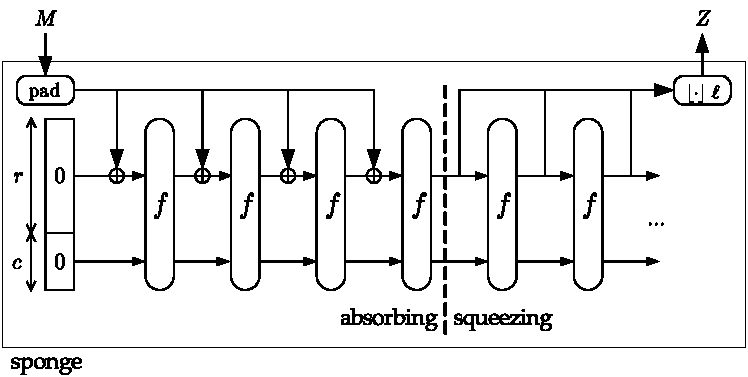
\includegraphics[width=\textwidth]{img/Sponge.pdf}
\caption{The sponge construction $\mathbf{sponge}[f,\mathbf{pad},r]$ \cite{Bertoni2011_SpongeFunctions}}
\label{fig:Sponge}
\end{figure}

The state of the sponge construction is split into two contiguous portions: the \emph{outer state}, which is accessible externally, and the \emph{inner state}, which is hidden.
The size of the outer state is given by the \emph{rate} $r$ and the size of the inner state is specified by the \emph{capacity} $c$.
The size of the entire state is $b = r + c$.
The speed of the construction partially relies on the rate, while the security is partially dependent on the capacity (see Section~\ref{subsec:SpongeSecurity}).

The padding function $\mathbf{pad}$ is first applied to $M$ to make it a multiple of $r$.
$M$ is then absorbed $r$ bits at a time.
More concretely, absorption is the process of XORing $r$-bit blocks into the state while interleaving with applications of the underlying sponge function $f$.
If the rate is increased, then more bits are absorbed at a time and thus the construction runs faster.
However, increasing the rate means that the capacity must decrease and so there is a clear trade-off between speed and security.
Squeezing consists of concatenating $r$ bits at a time to an output bitstring $Z$ that is truncated to $\ell$ bits.
The sponge function $f$ must be called once for each $r$ bits of output after the first full block.

\subsubsection{Simplified Sponge}
A padding function is required for the classical sponge construction in order to ensure that inputs can be reformed into bitstrings with length equal to a multiple of $r$. 
Two basic requirements of a padding function are that it be reversible and that it never produce identical outputs for different inputs.
We omit the lower level details of good padding functions here for brevity and refer the interested reader to \cite{Bertoni2011_SpongeFunctions} instead.

It is also useful, as we will see, to consider a sponge construction in which no padding function $\mathbf{pad}$ is required.
The parameterized interface for such a construction becomes
\begin{equation*}
Z = \mathbf{sponge}[f,r](M,\ell).
\end{equation*}
Alternatively, we can say that $\mathbf{pad}$ exists but it is trivially given as
\begin{equation*}
\mathbf{pad}(M) = M.
\end{equation*}
This lets us remain aligned with the original definition.
In either case, we assume that any necessary padding is performed at some higher level in the overall system.
This simplification allows us to focus more design effort towards the underlying sponge function $f$ and ignore the details of padding.

%For a more concrete treatment, we refer to the official SHA-3 hashing parameters:
\subsection{Applications}
\label{sec:SpongeApplications}
\subsubsection{Hashing}
The sponge construction was originally envisioned as a generalization of hash functions to functions with arbitrary length output.
Using the sponge construction for hashing is straightforward.
We denote a hash function by
\begin{equation*}
\mathbf{H} \from \Ztwo^* \to \Ztwo^{\ell}, 
\end{equation*}
where $\ell$ is the desired length of the message digest.
In this case, the message $M$ is padded and absorbed as usual.
After absorption completes, the construction switches to squeezing mode and the state is squeezed until a message digest of length $\ell$ is acquired.

Without any structural changes, several other applications can be derived from the sponge construction.
These following applications are of considerable relevance to the ultimate goal of authenticated encryption.

\subsubsection{MAC Generation}
A Message Authentication Code (MAC) function is essentially a keyed hash function.
We denote a MAC function under a given key $K$ and initialization vector $IV$ by
\begin{equation*}
\mathbf{MAC}_{K,IV} \from \Ztwo^k \times \Ztwo^v \times \Ztwo^* \to \Ztwo^{\ell},
\end{equation*}
where $k$ is the length of the key, $v$ is the length of the IV, and $\ell$ is the desired length of the tag (MAC).
In this case, $K||IV$ is absorbed first and then the padded message is absorbed directly after as usual.
Squeezing works the same as in a hash computation.
Note that the sponge construction is particularly attractive here (and in general with keyed modes) because to the sponge, there is no differentiation between the key, IV, and message data.
All input data is treated exactly the same, and thus the design remains simple.
This is in great contrast to traditional symmetric key cryptosystem design in which a key schedule is required.

\subsubsection{Bitstream Encryption}
The previous two direct applications of the sponge construction were characterized by long absorbing phases (assuming a long message) and short squeezing phases.
Bitstream encryption, i.e.\ using the sponge as a stream cipher, is characterized oppositely: absorbing is quick while squeezing is likely a much longer process.
We denote a stream cipher under a given key $K$ and initialization vector $IV$ by
\begin{equation*}
\mathbf{STREAM}_{K,IV} \from \Ztwo^k \times \Ztwo^v \to \Ztwo^{\infty},
\end{equation*}
where $k$ is the length of the key and $v$ is the length of the IV.
The codomain of such a stream cipher is the set of infinite bitstreams; in practice, the output is truncated to provide just enough keystream material to encrypt a given message $M$.
For this application, we simply absorb $K||IV$ and switch to the squeezing phase immediately.
Squeezing continues until a keystream is no longer needed.
The keystream is XORed with the message to produce the ciphertext.
Notice again how the overall structure of the algorithm remains the same as it was for its original application of hashing.

\subsection{Generic Security}
\label{subsec:SpongeSecurity}
It is typical to employ Kerckhoffs' principle when discussion the security of a cryptosystem.
This principle states that a cryptosystem should be secure regardless of any knowledge the adversary may have about the system (excluding the key).
Stated in a different way, the adversary is assumed to know every detail of the system except for the key \cite{Stinson2006_CTAP}.
Indeed, we even presume that an attacker has access to the cryptosystem.
In the case of a sponge construction, the adversary knows $f$ (and $f^{-1}$ if $f$ is a permutation).
The easiest way for him or her to gain knowledge about $f$ that may differentiate it from a random transformation is to simply make calls to it (and $f^{-1}$ if a permutation) \cite{Bertoni2011_SpongeFunctions}.

A \emph{random oracle} model is often useful as a framework for security proofs.
A random oracle (RO), which lies at the core of most sponge security proofs, is a theoretical ideal function
\begin{equation*}
\mathbf{RO} \from \mathbb{Z}_2^* \to \mathbb{Z}_2^{\infty}
\end{equation*}
such that every bit of the output, for every possible input, is chosen uniformly and independently. 
We state security proofs in the context of \emph{indistinguishability} in the random oracle model. 
We suppose that an adversary is able to query both a random oracle and the pseudorandom function (PRF) that we are testing.
The adversary then decides which of the systems is the PRF.
If it is ``hard'' for the adversary to do this, then the PRF is called indistinguishable from random. This is what we desire.
Hardness is given in terms of computational complexity and is subject to interpretation.
For example, if the adversary is able to accurately distinguish the two systems after only $2^{40}$ queries, then the PRF is not indistinguishable from random since a complexity of $2^{40}$ is computable with today's technology.
If, however, it takes a minimum of $2^{128}$ queries, then the system \emph{is} indistinguishable from random since this is not computable (i.e.\ such a computation would not finish within any reasonable time frame) and will not be computable in the foreseeable future \cite{Stinson2006_CTAP}.

The security of the sponge construction is based on the assumption that the underlying sponge function $f$ is secure.
That is, if $f$ is indistinguishable from random then so should be the sponge construction it is instantiated within.
Consequently, cryptographers designing a system based on the sponge construction need only be concerned with designing and cryptanalyzing a secure underlying function.
The sponge construction, when used properly, is said to be secure against \emph{generic attacks} -- attacks which do not exploit any specific properties of the underlying sponge function.
We call this the \emph{generic security} of the construction \cite{Bertoni2011_SpongeFunctions}.

\subsection{Security of Keyed Sponges}
The generic security of keyed constructions is higher than unkeyed.
For our purposes we are interested only in the security of the keyed sponge construction where a permutation is used for $f$. 

In \cite{Bertoni2011_SpongeKeyed} it is proven that the \emph{advantage} of distinguishing a keyed permutation-based sponge from a random oracle is
\begin{equation*}
\mathrm{max}\left( 
  1 - \mathrm{exp}\left(
    -\frac{\frac{M^2}{2}+2MN}{2^c}
  \right),
  \frac{N}{2^{|K|}}
\right),
\end{equation*}
where $M$ is the data complexity, $N$ is the time complexity, $c$ is the capacity, and $|K|$ is the size of the key.
The advantage is the probability of success of a generic attack.

We can take $N$ as the number of queries to the permutation $f$ and its inverse.
The data complexity $M$ is typically considered to be upper bounded by the implementation under a given key $K$.
For example, it is very reasonable and common practice to enforce that no more than, say, $M = 2^{40}$ operations be performed under a given key.
In \cite{Bertoni2011_SpongeKeyed} this exponent is called a \emph{usage exponent} and is denoted as $a$.
The assumption is made that $a \ll c / 2$ and the requirement (as is typical) is that no attacks are faster than a brute force search on the keyspace.
This ultimately leads to our metric of interest: a lower bound on the capacity $c$ such that there are no generic attacks (that allow differentiation from a random oracle) that are faster than exhausitive search.
This lower bound is given as
\begin{equation*} 
c \ge |K| + a + 1.
\end{equation*}

Jovanovic et.~al\ \cite{Jovanovic2014_Beyond} further improved on these results in 2014 by proving that the generic security level of keyed sponge constructions is lower bounded by 
\begin{equation*}
\mathrm{min}(2^{(r+c)/2}, 2^c, 2^{|K|}).
\end{equation*} 

%------------------------------
% SECTION:Duplex Construction
%------------------------------
\section{Duplex Construction}
The duplex construction is highly related to the sponge construction.
The main differences are that the duplex construction maintains state between calls and that there no longer exists a clear separation between the absorbing and squeezing phases.
Absorbing and squeezing happen essentially at the same time, hence ``duplexing''.
Other than this, switching from the sponge to the duplex construction is simply a matter of adjusting how inputs and outputs are handled.
The duplex mode has several applications, with authenticated encryption being the one of obvious interest to us.

\subsection{Duplex Parameters}
\begin{figure}[ht]
\centering
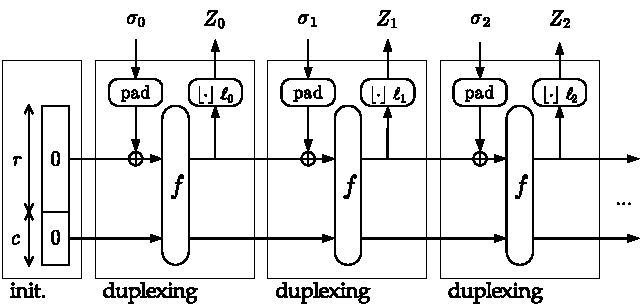
\includegraphics[width=\textwidth]{img/Duplex.pdf}
\caption{The duplex construction $\mathbf{duplex}[f,\mathbf{pad},r]$ \cite{Bertoni2011_SpongeFunctions}}
\label{fig:Duplex}
\end{figure}

Parameters for the duplex construction are mostly the same as for the sponge construction.
However, since the duplex construction maintains state, we build a \emph{duplex object} $D$ and make calls to it.
The function which processes inputs and produces outputs is called $\mathbf{duplexing}$:
\begin{equation*}
Z_i = D.\mathbf{duplexing}(\sigma_i,\ell_i)
\end{equation*}

Figure~\ref{fig:Duplex} shows the duplex construction.
The $i$-th input is denoted $\sigma_i$ and the $i$-th output is denoted $Z_i$, which is truncated to $\ell_i$ bits.
Inputs are absorbed and processed at the same time that outputs are squeezed.
For a duplex object it is possible to have an empty input or to not request an output.
A \emph{blank call} is a call to $\mathbf{duplexing}$ for which no input is provided ($|\sigma_i| = 0$).
A \emph{mute call} is a call for which no output is requested ($\ell_i = 0$).
The reasons for these types of calls will soon be apparent.

\subsubsection{Simplified Duplex}
In addition to the padding required for the sponge construction, the duplex construction also requires \emph{domain separation}.
This can be generally defined as a mechanism that allows differentiation between varying types of inputs (e.g.\ between header and body data).
In other words, it eliminates ambiguity on the receiving end that naturally arises from support for arbitrary length inputs.
The \Keccak designers use a \emph{frame bit} appended to the end of every input (see Figure~\ref{fig:DuplexAE}) in their original definition of the duplex construction \cite{Bertoni2012_Duplexing}.
The value of this bit toggles for every input type so that the receiver can differentiate between outputs.
Since the order of the inputs (and thus outputs) is always the same, a single frame bit is sufficient.

We also note that a frame bit is not the only way to achieve domain separation.
In general one can append a \emph{frame string}, denoted $\gamma_i$, to the end of every input.
The only requirements are that $|\gamma_i| \ge 1$ and $\gamma_i \ne \gamma_{i+1}$ for all $i$. 
For example, each frame string could be a byte instead of a single bit.

For the simplified duplex construction, we can make the assumption that both the padding and domain separation are accomplished at some higher level if needed.
This again allows us to focus more design effort towards the underlying sponge function.

\subsection{Duplex for Authenticated Encryption}
Authenticated encryption is easily achieved using the duplex construction.
It can be modeled under a given key $K$ as
\begin{equation*}
\mathbf{AE}_K \from \mathbb{Z}_2^k \times (\mathbb{Z}_2^*)^2 \to \mathbb{Z}_2^* \times \mathbb{Z}_2^{\ell},
\end{equation*}
where $k$ is the length of the key and $\ell$ is the length of the MAC desired.

Figure~\ref{fig:DuplexAE} shows the duplex construction being used in an AE use case.
Frame bits are shown, but recall that these are ignored in the simplified duplex construction.
First, we construct a duplex object $D$.
Then we absorb $K$ (or optionally $K||IV$) using one or more mute calls to $D.\mathbf{duplexing}$.
More that one mute call may be required if the length of the key exceeds the rate $r$.
We denote a header input to $D$ as $A$; these arbitrary length inputs are authenticated but not encrypted.
We denote a body input to $D$ as $B$; these arbitrary length inputs are both encrypted and authenticated.
$A$ inputs are absorbed using one or more mute calls to $D.\mathbf{duplexing}$.
$B$ inputs are absorbed in a similar fashion and then the keystream $Z$ is XORed with $B$ to produce the ciphertext $C$.
The tag $T$ is produced using a blank call to $D.\mathbf{duplexing}$ after all header and body inputs have been processed.

\begin{figure}[ht]
\centering
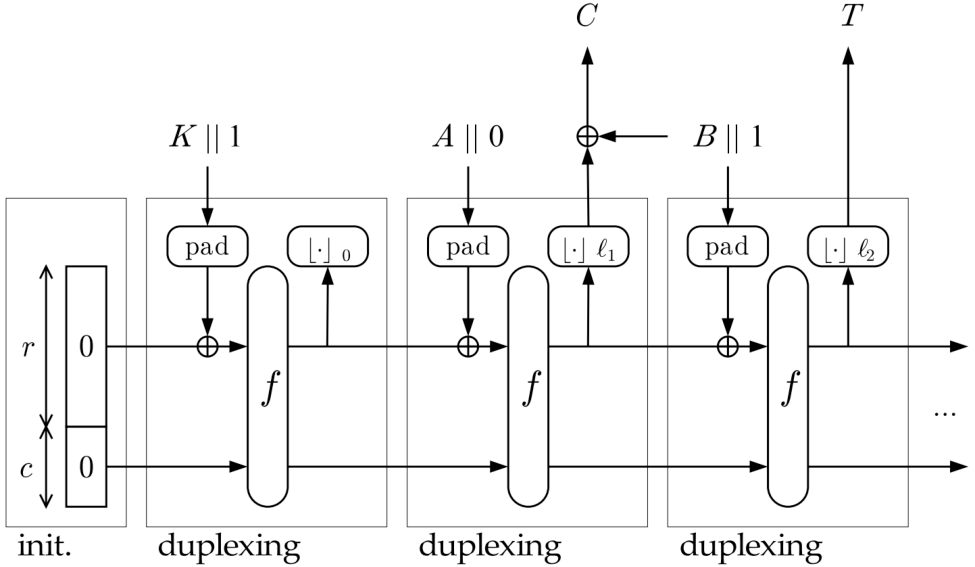
\includegraphics[width=\textwidth]{img/DuplexAE.pdf}
\caption{The duplex construction as used for authenticated encryption \cite{Bertoni2010_DuplexingSlides}}
\label{fig:DuplexAE}
\end{figure}

A more general case is shown in a slightly modified view in Figure~\ref{fig:DuplexAE_Expanded}. 
In this view, the duplex object $D$ is shown as a block and the different header and body inputs ($A_i$ and $B_i$ respectively) are absorbed over a series of calls to $D.\mathbf{duplexing}$. 
For example, the body $B$ consists of three blocks of size $r$ and so it requires three calls to be completely absorbed.
An intermediate tag is requested after the first header and body pair is processed and before the next header begins.
This is a very typical use case for e.g.\ network traffic.
The tag can be of arbitrary length.

\begin{figure}[ht]
\centering
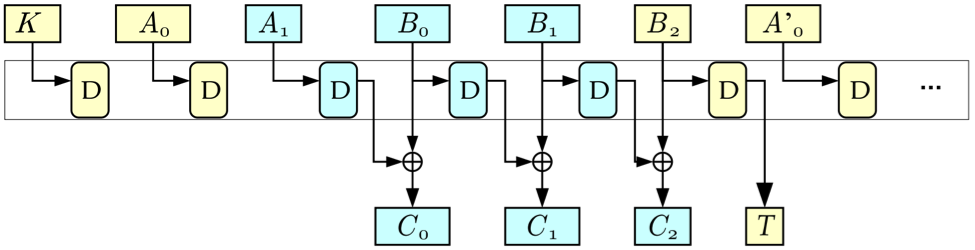
\includegraphics[width=\textwidth]{img/DuplexAE_Expanded.png}
\caption{The duplex construction as used for authenticated encryption (general case) \cite{Bertoni2010_DuplexingSlides}}
\label{fig:DuplexAE_Expanded}
\end{figure}

Clearly, the ciphertext and tags produced at any point depend on all of the previous inputs to $D$.
Intermediate tags can be produced if desired, since blank calls can be made at any time.
In summary, using the duplex construction for authenticated encryption provides the following advantages:
\begin{enumerate}
\item Easy to use
\item Single key required
\item Single-pass for encryption and authentication
\item Support for intermediate tags
\item Support for Additional Authenticated Data (AAD, or headers)
\item Secure against generic attacks
\item Ability to trade off speed and security by adjusting $r$
\end{enumerate}
The main disadvantage to using the duplex construction for AE is that it is not easily parallelizable as given here.
This should not be a concern most of the time since data (e.g.\ IP traffic) is often received and sent in a serial fashion for AE applications.
Compared to other methods of achieving AE, the duplex construction is clearly superior in the majority of applications.

\subsection{Security}
\label{sec:DuplexSecurity}
A reduction is used to prove the security of the duplex construction.
Any calls made to the duplex construction can be reduced to calls to the keyed sponge construction.
Therefore the security of the duplex depends on the security of the corresponding sponge, which can be shown to be secure against generic attacks.
For a concrete example, consider the $i$-th duplexing call to a duplex object $D$:
\begin{align*}
Z_i &= D.\mathbf{duplexing}(\sigma_i,\ell_i) \\
&= \mathbf{sponge}(\mathbf{pad}(\sigma_0)\ ||\ \mathbf{pad}(\sigma_1)\ ||\ \dots\ ||\ \mathbf{pad}(\sigma_i))
\end{align*}
Or in the case of a simplified duplex object $D$, we have:
\begin{align*}
Z_i &= D.\mathbf{duplexing}(\sigma_i,\ell_i) \\
&= \mathbf{sponge}(\sigma_0\ ||\ \sigma_1\ ||\ \dots\ ||\ \sigma_i),
\end{align*}
where $\sigma_i$ may be key, header, or body material.
Since this is true in general, it is clear that the duplex reduces to the sponge.
For a more rigorous proof, we refer to \cite{Bertoni2012_Duplexing}.

